\documentclass{beamer}

\usepackage{xcolor}
\usepackage{booktabs}
\usepackage{graphicx}
\usepackage{algorithm, algpseudocode}
\usepackage{textpos}
\usepackage{verbatim}
%\usepackage{algorithm,algorithmic}
\usepackage{tikz}

\setbeamertemplate{caption}[numbered]

\usepackage{tikz}
\usetikzlibrary{shapes.geometric}
\usetikzlibrary{arrows,shapes,trees}
\usetikzlibrary{calc,shapes.multipart,chains,arrows}

\usepackage{listings}
\lstset{language=Java,
    showspaces=false,
    showtabs=false,
    breaklines=true,
    showstringspaces=false,
    breakatwhitespace=true,
    commentstyle=\color{green},
    keywordstyle=\color{blue},
    stringstyle=\color{red},
    basicstyle=\footnotesize,
    moredelim=[is][\textcolor{grey}]{\%\%}{\%\%}
}

\definecolor{gray}{rgb}{0.4,0.4,0.4}
\definecolor{darkblue}{rgb}{0.0,0.0,0.6}
\definecolor{cyan}{rgb}{0.0,0.6,0.6}

\lstdefinelanguage{XML}{
    morestring=[b]",
    morestring=[s]{>}{<},
    morecomment=[s]{<?}{?>},
    stringstyle=\color{black},
    identifierstyle=\color{darkblue},
    keywordstyle=\color{cyan},
    morekeywords={xmlns,version,type}% list your attributes here
}

\usetheme{Madrid}
\useoutertheme{miniframes} % Alternatively: miniframes, infolines, split

% Setup the university's color pallette
\definecolor{UIUCorange}{RGB}{19, 41, 75} % UBC Blue (primary)
\definecolor{UIUCblue}{RGB}{232, 74, 39} % UBC Grey (secondary)

\setbeamercolor{palette primary}{bg=UIUCorange,fg=white}
\setbeamercolor{palette secondary}{bg=UIUCblue,fg=white}
\setbeamercolor{palette tertiary}{bg=UIUCblue,fg=white}
\setbeamercolor{palette quaternary}{bg=UIUCblue,fg=white}
\setbeamercolor{structure}{fg=UIUCorange} % itemize, enumerate, etc
\setbeamercolor{section in toc}{fg=UIUCblue} % TOC sections

\setbeamercolor{subsection in head/foot}{bg=UIUCorange,fg=UIUCblue}
\setbeamercolor{subsection in head/foot}{bg=UIUCorange,fg=UIUCblue}

\usepackage[utf8]{inputenc}


%Information to be included in the title page:
\title{\textbf{Linked Lists}}
\author{\textbf{}}
\institute[\textbf{UIUC}]{\textbf{}}
\date{}

\setbeamertemplate{title page}[default][colsep=-4bp,rounded=true]
\addtobeamertemplate{title page}{\vspace{3\baselineskip}}{}
\addtobeamertemplate{title page}{
    \begin{textblock*}{\paperwidth}(-1.0em, -1.2em)
        
\includegraphics[width=\paperwidth, height=\paperheight]{imgs/uiuc.jpg}
    \end{textblock*} 
}{}

\begin{document}

\tikzstyle{vertex}=[circle,fill=black!25,minimum size=20pt,inner sep=0pt]
\tikzstyle{selected vertex} = [vertex, fill=orange!24]
\tikzstyle{edge} = [draw,thick,-]
\tikzstyle{weight} = [font=\small]
\tikzstyle{selected edge} = [draw,line width=5pt,-,blue!50]
\tikzstyle{ignored edge} = [draw,line width=5pt,-,black!20]


\frame{\titlepage}

\begin{frame}
	\frametitle{Objectives}
    \begin{itemize}
        \item Understand the implementation of a LinkedList and it's ListNode class.
        \item Understand the process of implementing the following operations:
            \begin{itemize}
                \item Displaying the contents of the list.
                \item Searching for a given Node
                \item Removing Nodes
                \item Adding Nodes
            \end{itemize}
        \item You will extend these concepts in your mini-assignment in order to create a linked list with the following characteristics:
            \begin{itemize}
                \item Singly linked
                \item A head and tail pointers
            \end{itemize}
    \end{itemize}
\end{frame}

\section{Linked Lists}
\begin{frame}
    \begin{figure}
        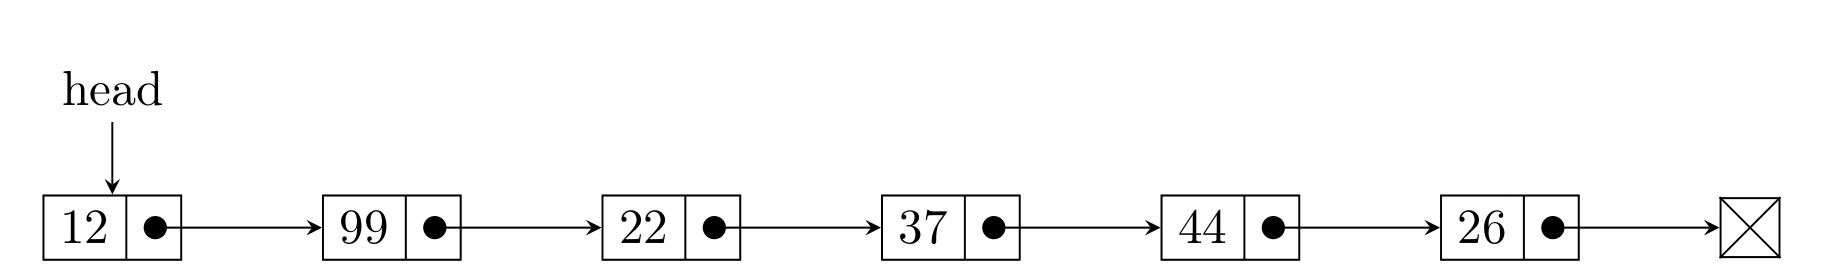
\includegraphics[width=\textwidth]{./imgs/linked-list.png}
    \end{figure}
    \vfill
    \textbf{Basic Operations:}\\
    \begin{itemize}
        \item \textbf{Add:} Adding operations add at either the front, middle, or end of the list.
        \item \textbf{Remove:} Remove removes a node either front, middle, or end of the list.
        \item \textbf{Search:} Search traverses the list, checks each node to see if it is the one we are looking for, and, if the node is found, returns a reference to it.
    \end{itemize}
\end{frame}

\section{ListNode Class}

\begin{frame}[fragile]
    \centering
    \vfill
    Off to the worksheet to implement the \lstinline|ListNode| class.
    \vfill
\end{frame}

\begin{frame}[fragile]
    \begin{minipage}{0.59\textwidth}
    \begin{lstlisting}[frame=trBL]
class ListNode{
    public int data;
    public ListNode next;

    ListNode(data){
        this.data = data;
        next = null;
    }
}
    \end{lstlisting}
    \end{minipage}
    \hfill
    \begin{minipage}{0.39\textwidth}
    \centering
    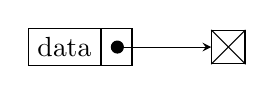
\begin{tikzpicture}[list/.style={rectangle split, rectangle split parts=2, draw, rectangle split horizontal}, >=stealth, start chain]
        \node[list,on chain] (A) {data};
        \node[on chain,draw,inner sep=6pt] (D) {};
        \draw (D.north east) -- (D.south west);
        \draw (D.north west) -- (D.south east);
        \draw[*->] let \p1 = (A.two), \p2 = (A.center) in (\x1,\y2) -- (D);
    \end{tikzpicture}\\
    \end{minipage}
\end{frame}

\section{LinkedList Class}
\begin{frame}[fragile]
    \frametitle{Nested vs Inner Classes}
    \begin{minipage}{0.45\textwidth}
    \begin{lstlisting}[frame=trBL]
class OuterClass{
    class InnerClass{
        //...
    }
}
    \end{lstlisting}
    \end{minipage}
    \hfill
    \begin{minipage}{0.49\textwidth}
    \begin{lstlisting}[frame=trBL]
class OuterClass{
    static class NestedClass{
        //...
    }
}
    \end{lstlisting}
    \end{minipage}
    \begin{itemize}
        \small
        \item \textbf{Inner Class:} Inner classes have no static modiers and therefore have: 1) access to all attributes and methods of the outer class and 2) cannot be instantiated unless the outerclass has been instantiated.
        \item \textbf{Nested Class:} Nested classes are declared with a \lstinline|static| modifier and are therefore independent of the outerclass.
    \end{itemize}
    \vfill
    \textbf{Key Point:} If the class needs access to things in the outerclass we use an \textit{inner class}. If it does not and we are encapsulating
    it as a design choice and the class is otherwise independent we use a \textit{nested class}.
\end{frame}

\begin{frame}[fragile]
    \begin{lstlisting}[frame=trBL]
class LinkedList{
    static class ListNode{/* ... */}

    ListNode head;
    int size;

    LinkedList(){
        head = null;
        size = 0;
    }

    /* Methods Below */
}
    \end{lstlisting}
    \begin{itemize}
        \item For your lab we will be setting up ListNodes as \textit{nested classes}.
        \item Design wise, they don't exist independently of the \lstinline|LinkedList| class.
        \item However, they don't need access to any of the attributes or methods of \lstinline|LinkedList|.
    \end{itemize}
\end{frame}

\section{Adding}
\begin{frame}[fragile]
    \frametitle{Manually Adding Nodes}
    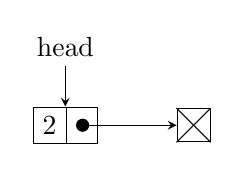
\begin{tikzpicture}[list/.style={rectangle split, rectangle split parts=2, draw, rectangle split horizontal}, >=stealth, start chain]

        \node[list,on chain] (A) {2};

        \node[on chain,draw,inner sep=6pt] (N1) {};
        \draw (N1.north east) -- (N1.south west);
        \draw (N1.north west) -- (N1.south east);

        \node[above of=A] (H) {head};

        \draw[*->] let \p1 = (A.two), \p2 = (A.center) in (\x1,\y2) -- (N1);

        \draw[->] (H) -- (A);

    \end{tikzpicture}\\
    \vfill
    \begin{lstlisting}[frame=trBL]
ListNode head = new ListNode(2);
    \end{lstlisting}

\end{frame}

\begin{frame}[fragile]
    \frametitle{Manually Adding Nodes}
    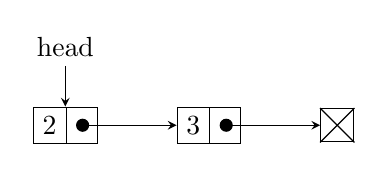
\begin{tikzpicture}[list/.style={rectangle split, rectangle split parts=2, draw, rectangle split horizontal}, >=stealth, start chain]

        \node[list,on chain] (A) {2};
        \node[list,on chain] (B) {3};

        \node[on chain,draw,inner sep=6pt] (N1) {};
        \draw (N1.north east) -- (N1.south west);
        \draw (N1.north west) -- (N1.south east);

        \node[above of=A] (H) {head};

        \draw[*->] let \p1 = (A.two), \p2 = (A.center) in (\x1,\y2) -- (B);
        \draw[*->] let \p1 = (B.two), \p2 = (B.center) in (\x1,\y2) -- (N1);

        \draw[->] (H) -- (A);

    \end{tikzpicture}\\
    \vfill
    \begin{lstlisting}[frame=trBL]
ListNode head = new ListNode(2);
head.next = new ListNode(3);
    \end{lstlisting}
\end{frame}

\begin{frame}[fragile]
    \frametitle{Manually Adding Nodes}
    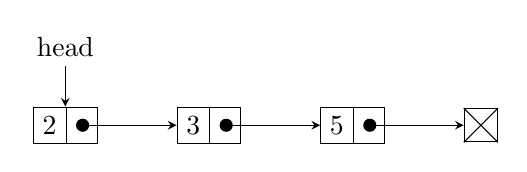
\begin{tikzpicture}[list/.style={rectangle split, rectangle split parts=2, draw, rectangle split horizontal}, >=stealth, start chain]

        \foreach \n\v in {A/2, B/3, C/5}{
            \node[list,on chain] (\n) {\v};
        }


        \node[on chain,draw,inner sep=6pt] (N1) {};
        \draw (N1.north east) -- (N1.south west);
        \draw (N1.north west) -- (N1.south east);

        \node[above of=A] (H) {head};

        \foreach \s\e in {A/B, B/C}{
            \draw[*->] let \p1 = (\s.two), \p2 = (\s.center) in (\x1,\y2) -- (\e);
        }

        \draw[*->] let \p1 = (C.two), \p2 = (C.center) in (\x1,\y2) -- (N1);
        \draw[->] (H) -- (A);

    \end{tikzpicture}\\
    \vfill
    \begin{lstlisting}[frame=trBL]
ListNode head = new ListNode(2);
head.next = new ListNode(3);
head.next.next = new ListNode(5);
    \end{lstlisting}
\end{frame}

\begin{frame}[fragile]
    \frametitle{Manually Adding Nodes}
    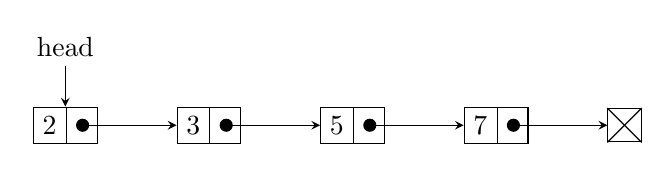
\begin{tikzpicture}[list/.style={rectangle split, rectangle split parts=2, draw, rectangle split horizontal}, >=stealth, start chain]
        \foreach \n\v in {A/2, B/3, C/5, D/7}{
            \node[list,on chain] (\n) {\v};
        }
        \node[on chain,draw,inner sep=6pt] (N1) {};
        \draw (N1.north east) -- (N1.south west);
        \draw (N1.north west) -- (N1.south east);
        \node[above of=A] (H) {head};
        \foreach \s\e in {A/B, B/C, C/D}{
            \draw[*->] let \p1 = (\s.two), \p2 = (\s.center) in (\x1,\y2) -- (\e);
        }
        \draw[*->] let \p1 = (D.two), \p2 = (B.center) in (\x1,\y2) -- (N1);
        \draw[->] (H) -- (A);
    \end{tikzpicture}\\
    \vfill
    \begin{lstlisting}[frame=trBL]
ListNode head = new ListNode(2);
head.next = new ListNode(3);
head.next.next = new ListNode(5);
head.next.next.next = new ListNode(7);
    \end{lstlisting}
\end{frame}

\begin{frame}
    \frametitle{Displaying a LinkedList}
    \centering
    \textit{Off to the worksheet to practice this!}
\end{frame}

\section{Displaying}
\begin{frame}[fragile]
    \frametitle{Displaying a LinkedList}
    \centering
    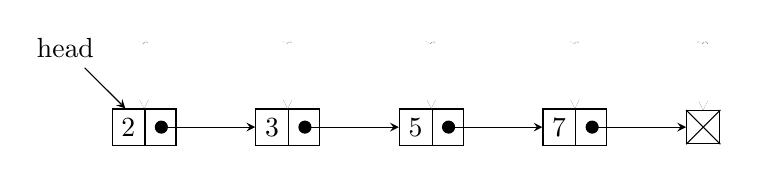
\begin{tikzpicture}[list/.style={rectangle split, rectangle split parts=2, draw, rectangle split horizontal}, >=stealth, start chain]
        \foreach \n\v in {A/2, B/3, C/5, D/7}{
            \node[list,on chain] (\n) {\v};
        }
        \node[on chain,draw,inner sep=6pt] (N1) {};
        \draw (N1.north east) -- (N1.south west);
        \draw (N1.north west) -- (N1.south east);
        \foreach \s\e in {A/B, B/C, C/D}{
            \draw[*->] let \p1 = (\s.two), \p2 = (\s.center) in (\x1,\y2) -- (\e);
        }
        \draw[*->] let \p1 = (D.two), \p2 = (B.center) in (\x1,\y2) -- (N1);

        \node[above of=A, xshift=-1.0cm] (H) {head};
        \draw[->] (H) -- (A);
        
        \pause
        \foreach \n in {A, B, C, D, N1}{
            \node[above of=\n] (FH) {tmp};
            \draw[->] (FH) -- (\n);
            \pause
            \node[above of=\n, color=white, line width=1mm] (FH) {\textbf{tmp}};
            \draw[->, color=white, line width=5mm] (FH) -- (\n);
        }
    \end{tikzpicture}\\
    \vfill
    \begin{itemize}
        \item We make a copy of the node referenced by \lstinline|head|
            \begin{itemize}
                \item \lstinline|ListNode tmp = head;|
            \end{itemize}
        \item We advance that reference by iteratively doing \lstinline|tmp = tmp.next|.
        \item Print the data in the node referenced by \lstinline|tmp|.
        \item We stop once \lstinline|tmp == null|.
    \end{itemize}
\end{frame}

%\begin{frame}[fragile]
%    \frametitle{Searching a LinkedList: Pseudocode}
%    \vfill
%    \centering
%    \begin{lstlisting}[frame=trBL]
%Procedure FindNode(Data)
%
%    /* Step 1: Get our head copy */
%    Tmp = Head
%
%    /* Step 2: Go through the list and find the thing */ 
%    While(Tmp != null)
%        Tmp = Tmp.Next
%        Print(Tmp.Data)
%    EndWhile
%
%EndProcedure
%    \end{lstlisting}
%    \vfill
%\end{frame}
%
%
%\begin{frame}
%    \frametitle{Worksheet: Displaying a LinkedList}
%    \vfill
%    \centering
%    Now we will implement this in the worksheet.
%    \vfill
%\end{frame}

%\section{Searching}
%\begin{frame}[fragile]
%    \frametitle{Searching a LinkedList}
%    \centering
%    \begin{tikzpicture}[list/.style={rectangle split, rectangle split parts=2, draw, rectangle split horizontal}, >=stealth, start chain]
%        \foreach \n\v in {A/2, B/3, C/5, D/7}{
%            \node[list,on chain] (\n) {\v};
%        }
%        \node[on chain,draw,inner sep=6pt] (N1) {};
%        \draw (N1.north east) -- (N1.south west);
%        \draw (N1.north west) -- (N1.south east);
%        \foreach \s\e in {A/B, B/C, C/D}{
%            \draw[*->] let \p1 = (\s.two), \p2 = (\s.center) in (\x1,\y2) -- (\e);
%        }
%        \draw[*->] let \p1 = (D.two), \p2 = (B.center) in (\x1,\y2) -- (N1);
%
%        \node[above of=A, xshift=-1.0cm] (H) {head};
%        \draw[->] (H) -- (A);
%        
%        \pause
%        \foreach \n in {A, B, C, D}{
%            \node[above of=\n] (FH) {tmp};
%            \draw[->] (FH) -- (\n);
%            \pause
%            \node[above of=\n, color=white, line width=1mm] (FH) {\textbf{tmp}};
%            \draw[->, color=white, line width=5mm] (FH) -- (\n);
%        }
%		\node[above of=D, color=black, line width=1mm] (FH) {\textbf{tmp}};
%		\draw[->, color=black] (FH) -- (D);
%    \end{tikzpicture}\\
%    \vfill
%    \begin{itemize}
%		\item Let's search the list for the node that contains 7
%        \item We make a copy of the reference to head.
%            \begin{itemize}
%                \item \lstinline|ListNode tmp = head;|
%            \end{itemize}
%        \item We advance that reference by iteratively doing \lstinline|tmp = tmp.next|.
%		\item Check each node to see if it's \lstinline|data| attribute matches what we're looking for:
%			\begin{itemize}
%				\item \lstinline|==| for primitives
%				\item \lstinline|.equals| for objects
%			\end{itemize}
%        \item We stop once we find what we're looking for or \lstinline|tmp == null|.
%    \end{itemize}
%\end{frame}

%\begin{frame}[fragile]
%    \frametitle{Searching a LinkedList: Pseudocode}
%    \vfill
%    \centering
%    \begin{lstlisting}[frame=trBL]
%Procedure FindNode(Data)
%
%    /* Step 1: Get our head copy */
%    Tmp = Head
%
%    /* Step 2: Go through the list and find the thing */ 
%    While(Tmp != null && !Tmp.GetData().Equals(Data))
%        Tmp = Tmp.Next
%    EndWhile
%
%    /* Step 3: Return Tmp's final value*/
%    Return Tmp
%
%EndProcedure
%    \end{lstlisting}
%    \vfill
%\end{frame}


\begin{frame}
    \frametitle{Worksheet: Displaying a LinkedList}
    \vfill
    \centering
    Now we will implement this in the worksheet.
    \vfill
\end{frame}



\section{Adding}
\begin{frame}
    \frametitle{Adding nodes to a LinkedList}
    \vfill
    \begin{itemize}
        \item \textbf{Case 0:} If the list is empty \lstinline|head=newNode|.
        \item There are three other cases for adding a node to a linked list if the list is not empty.
            \begin{itemize}
                \item \textbf{Case 1:} Adding to the end of the list.
                \item \textbf{Case 2:} Adding to the front of a list.
                \item \textbf{Case 3:} Adding in the middle of the list.
            \end{itemize}
        \item We'll cover all cases at a highlevel
        \item We'll cover case 1 in the worksheet as it's similar to displaying.
    \end{itemize}
    \vfill
\end{frame}


\begin{frame}[fragile]
    \frametitle{Case 1: Adding a Node to the End of a LinkedList}
    \centering
    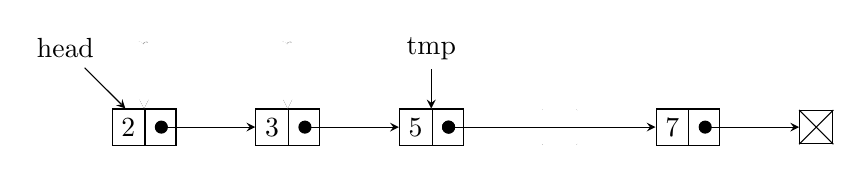
\begin{tikzpicture}[list/.style={rectangle split, rectangle split parts=2, draw, rectangle split horizontal}, >=stealth, start chain]
        \foreach \n\v in {A/2, B/3, C/5}{
            \node[list,on chain] (\n) {\v};
        }
        \node[on chain,draw,inner sep=6pt] (N1) {};
        \draw (N1.north east) -- (N1.south west);
        \draw (N1.north west) -- (N1.south east);
        \foreach \s\e in {A/B, B/C}{
            \draw[*->] let \p1 = (\s.two), \p2 = (\s.center) in (\x1,\y2) -- (\e);
        }
        \draw[*->] let \p1 = (C.two), \p2 = (C.center) in (\x1,\y2) -- (N1);

        \node[above of=A, xshift=-1.0cm] (H) {head};
        \draw[->] (H) -- (A);
        
        \pause
        \foreach \n in {A, B, C}{
            \node[above of=\n] (FH) {tmp};
            \draw[->] (FH) -- (\n);
            \pause
            \node[above of=\n, color=white, line width=1mm] (FH) {\textbf{tmp}};
            \draw[->, color=white, line width=5mm] (FH) -- (\n);
        }
        \node[above of=C] (FH) {tmp};
        \draw[->] (FH) -- (C);

        \node[list,on chain] (D) {7};
        \node[on chain,draw,inner sep=6pt] (N2) {};
        \draw (N2.north east) -- (N2.south west);
        \draw (N2.north west) -- (N2.south east);
        \draw[*->] let \p1 = (D.two), \p2 = (D.center) in (\x1,\y2) -- (N2);

        \pause
        \draw[line width=5mm,color=white] (N1.north east) -- (N1.south west);
        \draw[line width=5mm,color=white] (N1.north west) -- (N1.south east);
        \draw[*->] let \p1 = (C.two), \p2 = (C.center) in (\x1,\y2) -- (D);
        

    \end{tikzpicture}\\
    \vfill
    \begin{itemize}
        \item Find the end of the list by advancing \lstinline|tmp| until \lstinline|tmp.next == null|.
        \item Once we find that create a new node and \lstinline|tmp.next = newNode|
    \end{itemize}
\end{frame}

\begin{frame}[fragile]
    \frametitle{Case 1: Adding a Node to the End of a LinkedList Psuedocode}
    \vfill
    \centering
    \begin{lstlisting}[frame=trBL]
Procedure AddToEnd(Data)

    /* Step 1: Get our head copy */
    Tmp = Head

    /* Step 2: Go through the list and find the thing */ 
    While(Tmp.Next != Null)
        Tmp = Tmp.Next
    EndWhile

    Tmp.Next = new ListNode(Data)
    Size++
EndProcedure
    \end{lstlisting}
    \vfill
\end{frame}

\begin{frame}
    \frametitle{Worksheet: Adding a to the end of the list}
    \vfill
    \centering
    Now lets implement this method in a simplfied linked list class in the worksheet.
    \vfill
\end{frame}

\begin{frame}[fragile]
    \frametitle{Case 2: Adding to the Front}
    \centering
    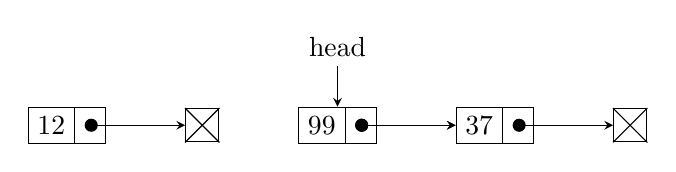
\begin{tikzpicture}[list/.style={rectangle split, rectangle split parts=2, draw, rectangle split horizontal}, >=stealth, start chain]

        \node[list,on chain] (A) {12};

        \node[on chain,draw,inner sep=6pt] (N1) {};
        \draw (N1.north east) -- (N1.south west);
        \draw (N1.north west) -- (N1.south east);

        \node[list,on chain] (B) {99};
        \node[list,on chain] (C) {37};
        \node[above of=B] (H) {head};
        \node[on chain,draw,inner sep=6pt] (D) {};
        \draw (D.north east) -- (D.south west);
        \draw (D.north west) -- (D.south east);
        \draw[*->] let \p1 = (A.two), \p2 = (A.center) in (\x1,\y2) -- (N1);
        \draw[*->] let \p1 = (B.two), \p2 = (B.center) in (\x1,\y2) -- (C);
        \draw[*->] let \p1 = (B.two), \p2 = (B.center) in (\x1,\y2) -- (C);
        \draw[*->] let \p1 = (C.two), \p2 = (C.center) in (\x1,\y2) -- (D);
        \draw[->] (H) -- (B);

    \end{tikzpicture}\\
    \vfill
    \begin{enumerate}
        \item Instantiate a new ListNode
    \end{enumerate}
\end{frame}

\begin{frame}
    \frametitle{Case 2: Adding to the Front}
    \centering
    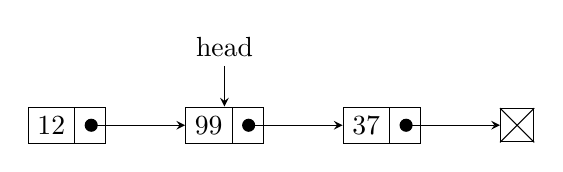
\begin{tikzpicture}[list/.style={rectangle split, rectangle split parts=2, draw, rectangle split horizontal}, >=stealth, start chain]

        \node[list,on chain] (A) {12};
        \node[list,on chain] (B) {99};
        \node[list,on chain] (C) {37};
        \node[above of=B] (H) {head};
        \node[on chain,draw,inner sep=6pt] (D) {};
        \draw (D.north east) -- (D.south west);
        \draw (D.north west) -- (D.south east);
        \draw[*->] let \p1 = (A.two), \p2 = (A.center) in (\x1,\y2) -- (B);
        \draw[*->] let \p1 = (B.two), \p2 = (B.center) in (\x1,\y2) -- (C);
        \draw[*->] let \p1 = (C.two), \p2 = (C.center) in (\x1,\y2) -- (D);
        \draw[->] (H) -- (B);

    \end{tikzpicture}\\
    \vfill
    \begin{enumerate}
        \item Instantiate a new ListNode
        \item Add the node to the front of the list by setting the new node's \lstinline|next| reference to the \lstinline|head|
    \end{enumerate}
\end{frame}

\begin{frame}
    \frametitle{Case 2: Adding to the Front}
    \centering
    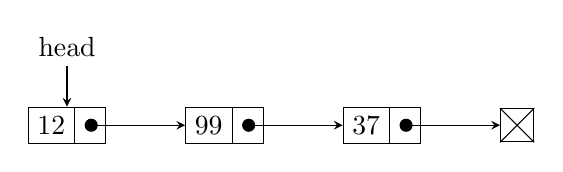
\begin{tikzpicture}[list/.style={rectangle split, rectangle split parts=2, draw, rectangle split horizontal}, >=stealth, start chain]

        \node[list,on chain] (A) {12};
        \node[list,on chain] (B) {99};
        \node[list,on chain] (C) {37};
        \node[above of=A] (H) {head};
        \node[on chain,draw,inner sep=6pt] (D) {};
        \draw (D.north east) -- (D.south west);
        \draw (D.north west) -- (D.south east);
        \draw[*->] let \p1 = (A.two), \p2 = (A.center) in (\x1,\y2) -- (B);
        \draw[*->] let \p1 = (B.two), \p2 = (B.center) in (\x1,\y2) -- (C);
        \draw[*->] let \p1 = (C.two), \p2 = (C.center) in (\x1,\y2) -- (D);
        \draw[->] (H) -- (A);

    \end{tikzpicture}\\
    \vfill
    \begin{enumerate}
        \item Instantiate a new ListNode
        \item Add the node to the front of the list by setting the \lstinline|next| reference 
        \item Update head attribute to reference the new node.
    \end{enumerate}
\end{frame}

\begin{frame}[fragile]
    \frametitle{Case 2: Adding a Node to the Front of a LinkedList Psuedocode}
    \vfill
    \centering
    \begin{lstlisting}[frame=trBL]
Procedure AddToFront(Data)
    /* Step 1: Check if our List is empty */
    If(Head is Null)
       Head = new ListNode(Data)
    Else
       NewNode = new ListNode(Data)

       /*Set the soon to be old head to the new one's next */
       NewNode.Next = Head

       /* Update the head attribute to be the new front */
       Head = NewNode
    EndIf
    Size++
EndProcedure
    \end{lstlisting}
    \vfill
\end{frame}



\begin{frame}
    \frametitle{Case 3: Adding to the Middle}
    \centering
    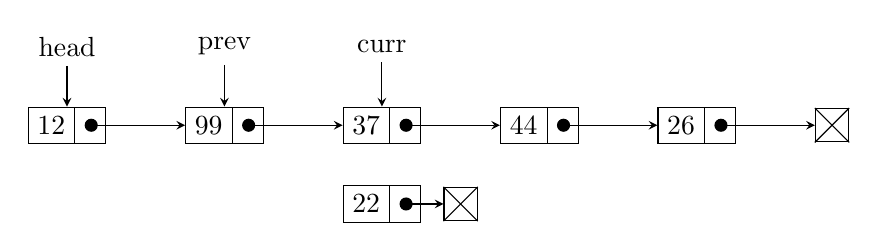
\begin{tikzpicture}[list/.style={rectangle split, rectangle split parts=2, draw, rectangle split horizontal}, >=stealth, start chain]

        \node[list,on chain] (A) {12};
        \node[list,on chain] (B) {99};
        \node[list,on chain] (C) {37};
        \node[list,on chain] (D) {44};
        \node[list,on chain] (E) {26};

        \node[list, below of=C] (New) {22};
        \node[draw,inner sep=6pt, right of=New] (N1) {};
        \draw (N1.north east) -- (N1.south west);
        \draw (N1.north west) -- (N1.south east);
        \draw[*->] let \p1 = (New.two), \p2 = (New.center) in (\x1,\y2) -- (N1);

        \node[above of=A] (H) {head};

        \node[above of=C] (Curr) {curr};
        \node[above of=B] (Prev) {prev};

        \node[on chain,draw,inner sep=6pt] (N) {};
        \draw (N.north east) -- (N.south west);
        \draw (N.north west) -- (N.south east);

        \draw[*->] let \p1 = (A.two), \p2 = (A.center) in (\x1,\y2) -- (B);
        \draw[*->] let \p1 = (B.two), \p2 = (B.center) in (\x1,\y2) -- (C);
        \draw[*->] let \p1 = (C.two), \p2 = (C.center) in (\x1,\y2) -- (D);
        \draw[*->] let \p1 = (D.two), \p2 = (D.center) in (\x1,\y2) -- (E);
        \draw[*->] let \p1 = (E.two), \p2 = (E.center) in (\x1,\y2) -- (N);

        \draw[->] (Curr) -- (C);
        \draw[->] (Prev) -- (B);

        \draw[->] (H) -- (A);

    \end{tikzpicture}\\
    \vfill
    \begin{enumerate}
        \item We have two pointers one that is similar to tmp from the previous example (\lstinline|curr|) and one that follows it (\lstinline|prev|).
        \item Advance \lstinline|curr| and \lstinline|prev| until we find the position at which we want to insert.
        \item Create a new node.
    \end{enumerate}
\end{frame}

\begin{frame}
    \frametitle{Case 3: Adding to the Middle}
    \centering
    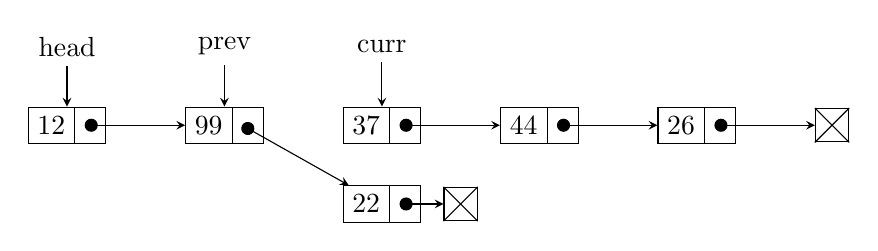
\begin{tikzpicture}[list/.style={rectangle split, rectangle split parts=2, draw, rectangle split horizontal}, >=stealth, start chain]

        \node[list,on chain] (A) {12};
        \node[list,on chain] (B) {99};
        \node[list,on chain] (C) {37};
        \node[list,on chain] (D) {44};
        \node[list,on chain] (E) {26};

        \node[list, below of=C] (New) {22};
        \node[draw,inner sep=6pt, right of=New] (N1) {};
        \draw (N1.north east) -- (N1.south west);
        \draw (N1.north west) -- (N1.south east);
        \draw[*->] let \p1 = (New.two), \p2 = (New.center) in (\x1,\y2) -- (N1);

        \node[above of=A] (H) {head};

        \node[above of=C] (Curr) {curr};
        \node[above of=B] (Prev) {prev};

        \node[on chain,draw,inner sep=6pt] (N) {};
        \draw (N.north east) -- (N.south west);
        \draw (N.north west) -- (N.south east);

        \draw[*->] let \p1 = (A.two), \p2 = (A.center) in (\x1,\y2) -- (B);
        \draw[*->] let \p1 = (B.two), \p2 = (B.center) in (\x1,\y2) -- (New);
        \draw[*->] let \p1 = (C.two), \p2 = (C.center) in (\x1,\y2) -- (D);
        \draw[*->] let \p1 = (D.two), \p2 = (D.center) in (\x1,\y2) -- (E);
        \draw[*->] let \p1 = (E.two), \p2 = (E.center) in (\x1,\y2) -- (N);

        \draw[->] (Curr) -- (C);
        \draw[->] (Prev) -- (B);

        \draw[->] (H) -- (A);

    \end{tikzpicture}\\
    \vfill
    \begin{enumerate}
        \item We have two pointers one that is similar to tmp from the previous example (\lstinline|curr|) and one that follows it (\lstinline|prev|).
        \item Advance \lstinline|curr| and \lstinline|prev| until we find the position at which we want to insert.
        \item Create a new node.
        \item Set the \lstinline|prev.next| to point to the new node.
    \end{enumerate}
\end{frame}

\begin{frame}
    \frametitle{Case 3: Adding to the Middle}
    \centering
    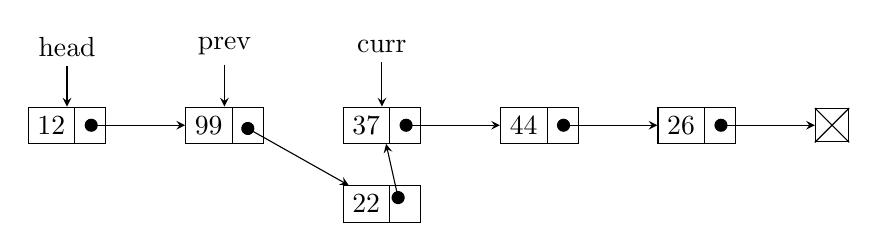
\begin{tikzpicture}[list/.style={rectangle split, rectangle split parts=2, draw, rectangle split horizontal}, >=stealth, start chain]

        \node[list,on chain] (A) {12};
        \node[list,on chain] (B) {99};
        \node[list,on chain] (C) {37};
        \node[list,on chain] (D) {44};
        \node[list,on chain] (E) {26};

        \node[list, below of=C] (New) {22};

        \node[above of=A] (H) {head};

        \node[above of=C] (Curr) {curr};
        \node[above of=B] (Prev) {prev};

        \node[on chain,draw,inner sep=6pt] (N) {};
        \draw (N.north east) -- (N.south west);
        \draw (N.north west) -- (N.south east);

        \draw[*->] let \p1 = (A.two), \p2 = (A.center) in (\x1,\y2) -- (B);
        \draw[*->] let \p1 = (B.two), \p2 = (B.center) in (\x1,\y2) -- (New);
        \draw[*->] let \p1 = (New.two), \p2 = (New.center) in (\x1,\y2) -- (C);
        \draw[*->] let \p1 = (C.two), \p2 = (C.center) in (\x1,\y2) -- (D);
        \draw[*->] let \p1 = (D.two), \p2 = (D.center) in (\x1,\y2) -- (E);
        \draw[*->] let \p1 = (E.two), \p2 = (E.center) in (\x1,\y2) -- (N);

        \draw[->] (Curr) -- (C);
        \draw[->] (Prev) -- (B);

        \draw[->] (H) -- (A);


    \end{tikzpicture}\\
    \vfill
    \begin{enumerate}
        \item We have two pointers one that is similar to tmp from the previous example (\lstinline|curr|) and one that follows it (\lstinline|prev|).
        \item Advance \lstinline|curr| and \lstinline|prev| until we find the position at which we want to insert.
        \item Create a new node.
        \item Set the \lstinline|prev.next| to point to the new node.
        \item Set the new node's \lstinline|next| pointer equal to \lstinline|curr|.
    \end{enumerate}
\end{frame}

\begin{frame}[fragile]
    \frametitle{Case 3: Adding a Node to the Middle Psuedocode}
    \vfill
    \centering
    \begin{lstlisting}[frame=trBL]
Procedure AddToMiddle(Index, Data)
    If(Index not Valid) Return/Error

    Prev = Null
    Curr = Head
    
    For(1 to Index)
        Prev = Curr
        Curr = Curr.Next
    EndFor
    
    NewNode = new ListNode(Data)
    Prev.Next = NewNode
    NewNode.Next = Curr
    Size++
EndProcedure
    \end{lstlisting}
    \vfill
\end{frame}



\section{Removing}

\begin{frame}
    \frametitle{Removing nodes from a LinkedList}
    \vfill
    \begin{itemize}
        \item \textbf{Case 0:} Again, if the list is empty we need to check if there is anything to remove.
        \item We have the same three cases when removing a node to a linked list:
            \begin{itemize}
                \item \textbf{Case 1:} Adding to the front of a list.
                \item \textbf{Case 2:} Adding to the end of the list.
                \item \textbf{Case 3:} Adding in the middle of the list.
            \end{itemize}
        \item We'll cover all cases at a highlevel
        \item We'll cover case 1 in the worksheet as it's similar to displaying.
    \end{itemize}
    \vfill
\end{frame}

\begin{frame}
    \frametitle{Case 1: Remove from Front}
    \centering
    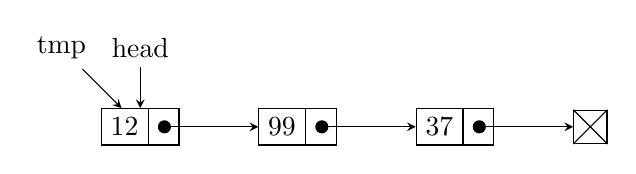
\begin{tikzpicture}[list/.style={rectangle split, rectangle split parts=2, draw, rectangle split horizontal}, >=stealth, start chain]

        \node[list,on chain] (A) {12};
        \node[list,on chain] (B) {99};
        \node[list,on chain] (C) {37};
        \node[above of=A] (H) {head};
        \node[left of=H] (Tmp) {tmp};
        \node[on chain,draw,inner sep=6pt] (D) {};
        \draw (D.north east) -- (D.south west);
        \draw (D.north west) -- (D.south east);
        \draw[*->] let \p1 = (A.two), \p2 = (A.center) in (\x1,\y2) -- (B);
        \draw[*->] let \p1 = (B.two), \p2 = (B.center) in (\x1,\y2) -- (C);
        \draw[*->] let \p1 = (C.two), \p2 = (C.center) in (\x1,\y2) -- (D);
        \draw[->] (H) -- (A);
        \draw[->] (Tmp) -- (A);

    \end{tikzpicture}\\
    \vfill
    \begin{enumerate}
        \item Make a \lstinline|tmp|reference to the same node referenced by the head.
    \end{enumerate}
\end{frame}

\begin{frame}
    \frametitle{Case 1: Remove from Front}
    \centering
    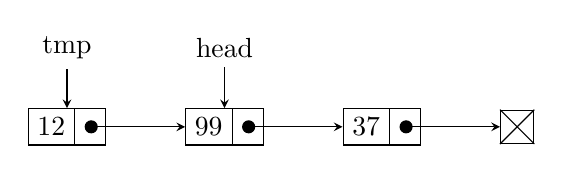
\begin{tikzpicture}[list/.style={rectangle split, rectangle split parts=2, draw, rectangle split horizontal}, >=stealth, start chain]

        \node[list,on chain] (A) {12};
        \node[list,on chain] (B) {99};
        \node[list,on chain] (C) {37};
        \node[above of=B] (H) {head};
        \node[above of=A] (Tmp) {tmp};
        \node[on chain,draw,inner sep=6pt] (D) {};
        \draw (D.north east) -- (D.south west);
        \draw (D.north west) -- (D.south east);
        \draw[*->] let \p1 = (A.two), \p2 = (A.center) in (\x1,\y2) -- (B);
        \draw[*->] let \p1 = (B.two), \p2 = (B.center) in (\x1,\y2) -- (C);
        \draw[*->] let \p1 = (C.two), \p2 = (C.center) in (\x1,\y2) -- (D);
        \draw[->] (H) -- (B);
        \draw[->] (Tmp) -- (A);

    \end{tikzpicture}\\
    \vfill
    \begin{enumerate}
        \item Make a \lstinline|tmp| reference to the same node referenced by the head.
        \item Advance the \lstinline|head|.
    \end{enumerate}
\end{frame}

\begin{frame}
    \frametitle{Case 1: Remove from Front}
    \centering
    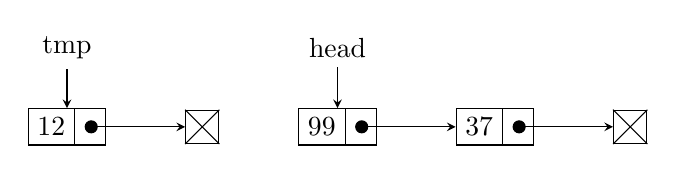
\begin{tikzpicture}[list/.style={rectangle split, rectangle split parts=2, draw, rectangle split horizontal}, >=stealth, start chain]

        \node[list,on chain] (A) {12};

        \node[on chain,draw,inner sep=6pt] (N1) {};
        \draw (N1.north east) -- (N1.south west);
        \draw (N1.north west) -- (N1.south east);

        \node[list,on chain] (B) {99};
        \node[list,on chain] (C) {37};
        \node[above of=B] (H) {head};
        \node[above of=A] (Tmp) {tmp};


        \node[on chain,draw,inner sep=6pt] (D) {};
        \draw (D.north east) -- (D.south west);
        \draw (D.north west) -- (D.south east);
        \draw[*->] let \p1 = (A.two), \p2 = (A.center) in (\x1,\y2) -- (N1);
        \draw[*->] let \p1 = (B.two), \p2 = (B.center) in (\x1,\y2) -- (C);
        \draw[*->] let \p1 = (C.two), \p2 = (C.center) in (\x1,\y2) -- (D);
        \draw[->] (H) -- (B);
        \draw[->] (Tmp) -- (A);

    \end{tikzpicture}\\
    \vfill
    \begin{enumerate}
        \item Make a \lstinline|tmp| variable that references the same node referenced by the head.
        \item Advance the \lstinline|head|.
        \item Set \lstinline|tmp.next| equal to null.
    \end{enumerate}
\end{frame}

\begin{frame}[fragile]
    \frametitle{Case 1: Remove from Front Psuedocode}
    \begin{lstlisting}[frame=trBL]
Procedure RemoveFromFront()
    If(Head is Null)
        Return/Error
    EndIf
    Tmp = Head
    Head = Head.Next
    Tmp.Next = Null
    Size--
EndProcedure
    \end{lstlisting}
\end{frame}


\begin{frame}
    \frametitle{Case 2: Remove from Back}
    \textbf{Before:}\\
    \vfill
    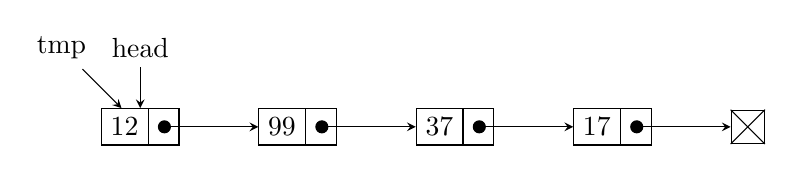
\begin{tikzpicture}[list/.style={rectangle split, rectangle split parts=2, draw, rectangle split horizontal}, >=stealth, start chain]

        \node[list,on chain] (A) {12};
        \node[list,on chain] (B) {99};
        \node[list,on chain] (C) {37};
        \node[list,on chain] (D) {17};

        \node[above of=A] (H) {head};
        \node[left of=H] (Tmp) {tmp};

        \node[on chain,draw,inner sep=6pt] (N) {};
        \draw (N.north east) -- (N.south west);
        \draw (N.north west) -- (N.south east);
        \draw[*->] let \p1 = (A.two), \p2 = (A.center) in (\x1,\y2) -- (B);
        \draw[*->] let \p1 = (B.two), \p2 = (B.center) in (\x1,\y2) -- (C);
        \draw[*->] let \p1 = (C.two), \p2 = (C.center) in (\x1,\y2) -- (D);
        \draw[*->] let \p1 = (D.two), \p2 = (D.center) in (\x1,\y2) -- (N);

        \draw[->] (H) -- (A);
        \draw[->] (Tmp) -- (A);

    \end{tikzpicture}\\
    \vfill
    \hline
    \vfill
    \textbf{After:}\\
    \vfill
    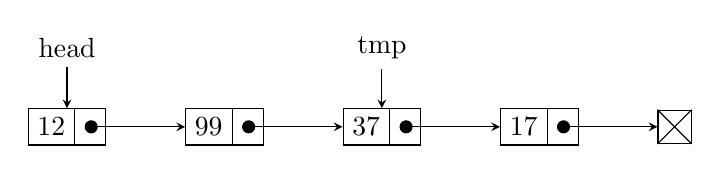
\begin{tikzpicture}[list/.style={rectangle split, rectangle split parts=2, draw, rectangle split horizontal}, >=stealth, start chain]

        \node[list,on chain] (A) {12};
        \node[list,on chain] (B) {99};
        \node[list,on chain] (C) {37};
        \node[list,on chain] (D) {17};

        \node[above of=A] (H) {head};
        \node[above of=C] (Tmp) {tmp};

        \node[on chain,draw,inner sep=6pt] (N) {};
        \draw (N.north east) -- (N.south west);
        \draw (N.north west) -- (N.south east);
        \draw[*->] let \p1 = (A.two), \p2 = (A.center) in (\x1,\y2) -- (B);
        \draw[*->] let \p1 = (B.two), \p2 = (B.center) in (\x1,\y2) -- (C);
        \draw[*->] let \p1 = (C.two), \p2 = (C.center) in (\x1,\y2) -- (D);
        \draw[*->] let \p1 = (D.two), \p2 = (D.center) in (\x1,\y2) -- (N);

        \draw[->] (H) -- (A);
        \draw[->] (Tmp) -- (C);

    \end{tikzpicture}\\
    \vfill
    \begin{enumerate}
        \item Find the second to last node in the list by iterating until either:
            \begin{enumerate}
                \item tmp.next.next == null
                \item you've iterated size - 2 times
            \end{enumerate}
    \end{enumerate}
\end{frame}


\begin{frame}
    \frametitle{Case 2: Remove from Back}
    \centering
    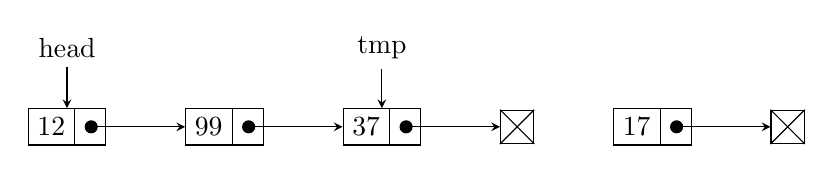
\begin{tikzpicture}[list/.style={rectangle split, rectangle split parts=2, draw, rectangle split horizontal}, >=stealth, start chain]

        \node[list,on chain] (A) {12};
        \node[list,on chain] (B) {99};
        \node[list,on chain] (C) {37};

        \node[on chain,draw,inner sep=6pt] (N1) {};
        \draw (N1.north east) -- (N1.south west);
        \draw (N1.north west) -- (N1.south east);

        \node[list,on chain] (D) {17};

        \node[above of=A] (H) {head};
        \node[above of=C] (Tmp) {tmp};

        \node[on chain,draw,inner sep=6pt] (N2) {};
        \draw (N2.north east) -- (N2.south west);
        \draw (N2.north west) -- (N2.south east);
        \draw[*->] let \p1 = (A.two), \p2 = (A.center) in (\x1,\y2) -- (B);
        \draw[*->] let \p1 = (B.two), \p2 = (B.center) in (\x1,\y2) -- (C);
        \draw[*->] let \p1 = (C.two), \p2 = (C.center) in (\x1,\y2) -- (N1);
        \draw[*->] let \p1 = (D.two), \p2 = (D.center) in (\x1,\y2) -- (N2);

        \draw[->] (H) -- (A);
        \draw[->] (Tmp) -- (C);

    \end{tikzpicture}\\
    \vfill
    \begin{enumerate}
        \item Find the second to last node in the list.
        \item Set it's reference to the next node equal to \lstinline|null|.
    \end{enumerate}
\end{frame}

\begin{frame}
    \frametitle{Case 2: Remove from end}
    There are three subcases to consider:
    \begin{enumerate}
        \item The list is empty (i.e., \lstinline|head == null|) so we can't remove.
        \begin{enumerate}
            \item \textbf{Solution: } Return or throw an exception.
        \end{enumerate}
        \item There is only one element in the list (i.e., head.next == null or size == 1)
        \begin{enumerate}
            \item \textbf{Solution: } Just set the head equal to null.
        \end{enumerate}
        \item There are more than two elements. 
        \begin{enumerate}
            \item \textbf{Solution: } We just went over that
        \end{enumerate}
    \end{enumerate}
\end{frame}


\begin{frame}[fragile]
    \frametitle{Case 2: Remove from Back Psuedocode}
    \begin{lstlisting}[frame=trBL]
Procedure RemoveFromBack(i)
    If(Head is Null)
        Return/Error
    ElseIf(Head.Next is Null)
        Head = Null
    Else
        Tmp = Head
        While(Tmp.Next.Next != Null)
            Tmp = Tmp.Next
        EndWhile
        Tmp.Next = Null
    EndIf
    Size--
EndProcedure
    \end{lstlisting}
\end{frame}

\begin{frame}[fragile]
    \frametitle{Case 3: Remove from Middle}
    \centering
    \resizebox{\textwidth}{!}{
    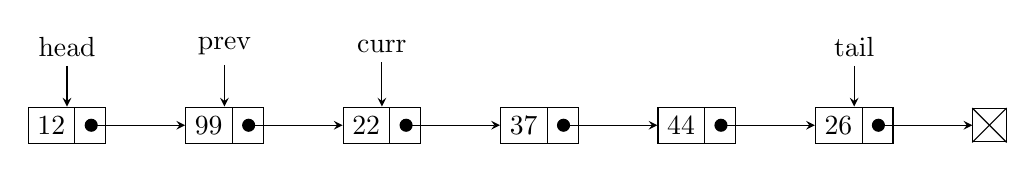
\begin{tikzpicture}[list/.style={rectangle split, rectangle split parts=2, draw, rectangle split horizontal}, >=stealth, start chain]

        \node[list,on chain] (A) {12};
        \node[list,on chain] (B) {99};
        \node[list,on chain] (C) {22};
        \node[list,on chain] (D) {37};
        \node[list,on chain] (E) {44};
        \node[list,on chain] (F) {26};


        \node[above of=A] (H) {head};
        \node[above of=F] (T) {tail};

        \node[above of=C] (Curr) {curr};
        \node[above of=B] (Prev) {prev};

        \node[on chain,draw,inner sep=6pt] (N) {};
        \draw (N.north east) -- (N.south west);
        \draw (N.north west) -- (N.south east);

        \draw[*->] let \p1 = (A.two), \p2 = (A.center) in (\x1,\y2) -- (B);
        \draw[*->] let \p1 = (B.two), \p2 = (B.center) in (\x1,\y2) -- (C);
        \draw[*->] let \p1 = (C.two), \p2 = (C.center) in (\x1,\y2) -- (D);
        \draw[*->] let \p1 = (D.two), \p2 = (D.center) in (\x1,\y2) -- (E);
        \draw[*->] let \p1 = (E.two), \p2 = (E.center) in (\x1,\y2) -- (F);
        \draw[*->] let \p1 = (F.two), \p2 = (F.center) in (\x1,\y2) -- (N);

        \draw[->] (Curr) -- (C);
        \draw[->] (Prev) -- (B);

        \draw[->] (H) -- (A);
        \draw[->] (T) -- (F);

    \end{tikzpicture}}\\
    \textbf{Step 1: Search for and find a reference to the node you want to remove and the node that precedes it.}
    \vfill
    \begin{lstlisting}[frame=trBL]
/* Step 1: Start at the beginning */
Prev = Null
Curr = Head

/* Walk through the list */
While(We havent found our thing/spot)
    Prev = Curr
    Curr = Curr.Next
EndWhile
    \end{lstlisting}
\end{frame}

\begin{frame}[fragile]
    \frametitle{Case 3: Remove from Middle}
    \centering
    \resizebox{\textwidth}{!}{
    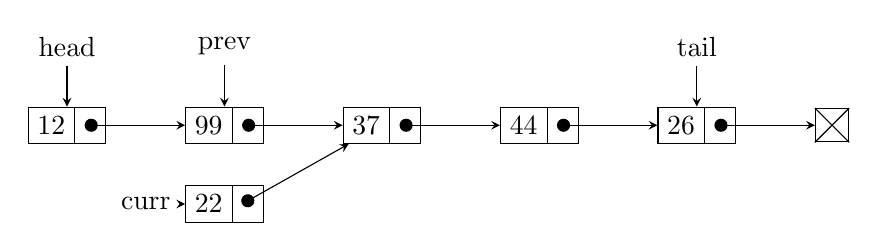
\begin{tikzpicture}[list/.style={rectangle split, rectangle split parts=2, draw, rectangle split horizontal}, >=stealth, start chain]

        \node[list,on chain] (A) {12};
        \node[list,on chain] (B) {99};
        \node[list, below of=B] (C) {22};
        \node[list,on chain] (D) {37};
        \node[list,on chain] (E) {44};
        \node[list,on chain] (F) {26};

dfksdfljkdfjkl
        \node[above of=A] (H) {head};
        \node[above of=F] (T) {tail};

        \node[left of=C] (Curr) {curr};
        \node[above of=B] (Prev) {prev};

        \node[on chain,draw,inner sep=6pt] (N) {};
        \draw (N.north east) -- (N.south west);
        \draw (N.north west) -- (N.south east);

        \draw[*->] let \p1 = (A.two), \p2 = (A.center) in (\x1,\y2) -- (B);
        \draw[*->] let \p1 = (B.two), \p2 = (B.center) in (\x1,\y2) -- (D);
        \draw[*->] let \p1 = (C.two), \p2 = (C.center) in (\x1,\y2) -- (D);
        \draw[*->] let \p1 = (D.two), \p2 = (D.center) in (\x1,\y2) -- (E);
        \draw[*->] let \p1 = (E.two), \p2 = (E.center) in (\x1,\y2) -- (F);
        \draw[*->] let \p1 = (F.two), \p2 = (F.center) in (\x1,\y2) -- (N);

        \draw[->] (Curr) -- (C);
        \draw[->] (Prev) -- (B);

        \draw[->] (H) -- (A);
        \draw[->] (T) -- (F);

    \end{tikzpicture}}\\
    \textbf{Step 2: Update previous node's next node to be the current nodes next node.}
    \vfill
    \begin{lstlisting}[frame=trBL]
/* Remove the element */
Prev.Next = Curr.Next // <--- Here
Curr.Next = Null
    \end{lstlisting}
\end{frame}

\begin{frame}[fragile]
    \frametitle{Case 2: Remove from Middle}
    \centering
    \resizebox{\textwidth}{!}{
    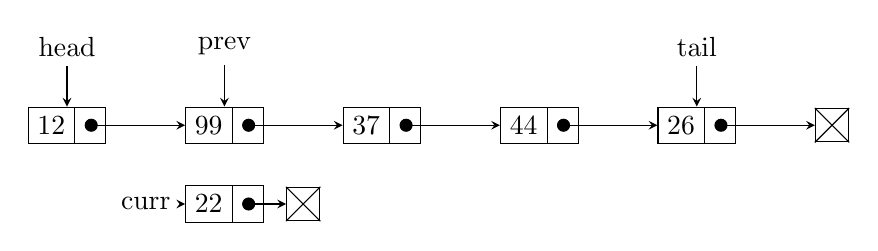
\begin{tikzpicture}[list/.style={rectangle split, rectangle split parts=2, draw, rectangle split horizontal}, >=stealth, start chain]

        \node[list,on chain] (A) {12};
        \node[list,on chain] (B) {99};
        \node[list, below of=B] (C) {22};
        \node[list,on chain] (D) {37};
        \node[list,on chain] (E) {44};
        \node[list,on chain] (F) {26};


        \node[above of=A] (H) {head};
        \node[above of=F] (T) {tail};

        \node[left of=C] (Curr) {curr};
        \node[above of=B] (Prev) {prev};

        \node[on chain,draw,inner sep=6pt] (N) {};
        \draw (N.north east) -- (N.south west);
        \draw (N.north west) -- (N.south east);


        \node[right of=C, draw,inner sep=6pt] (N1) {};
        \draw (N1.north east) -- (N1.south west);
        \draw (N1.north west) -- (N1.south east);

        \draw[*->] let \p1 = (A.two), \p2 = (A.center) in (\x1,\y2) -- (B);
        \draw[*->] let \p1 = (B.two), \p2 = (B.center) in (\x1,\y2) -- (D);
        \draw[*->] let \p1 = (C.two), \p2 = (C.center) in (\x1,\y2) -- (N1);
        \draw[*->] let \p1 = (D.two), \p2 = (D.center) in (\x1,\y2) -- (E);
        \draw[*->] let \p1 = (E.two), \p2 = (E.center) in (\x1,\y2) -- (F);
        \draw[*->] let \p1 = (F.two), \p2 = (F.center) in (\x1,\y2) -- (N);

        \draw[->] (Curr) -- (C);
        \draw[->] (Prev) -- (B);

        \draw[->] (H) -- (A);
        \draw[->] (T) -- (F);


    \end{tikzpicture}}\\
    \textbf{Step 3: Null out the current nodes next node to fully remove it from the list}
    \vfill
    \begin{lstlisting}[frame=trBL]
/* Remove the element */
Prev.Next = Curr.Next 
Curr.Next = Null // <--- Here 
    \end{lstlisting}

\end{frame}

\begin{frame}[fragile]
    \frametitle{Case 3: Remove from Middle Psuedocode}
    \begin{lstlisting}[frame=trBL]
Procedure RemoveFromMiddle(i)
    /* Check if it's valid */
    If(i < 1 || i > size - 2)
        Return/Error
    EndIf

    Prev = Null
    Tmp = Head

    For(0 to i)
        Prev = Tmp
        Tmp = Tmp.Next
    EndFor

    Prev.Next = Tmp.Next
    Tmp.Next = Null
EndProcedure
    \end{lstlisting}
\end{frame}

\section{Generic LinkedList}
\begin{frame}[fragile]
    \frametitle{Generic Linked List Template}
    \vfill
    \begin{lstlisting}[frame=trBL, basicstyle=\tiny]
public class GList<E>{

    public class GListNode<E>{
        /* Attributes */
    }
    
    public GList(){
    
    }
    
    
    public void addNode(E data){

    }
    
    public void displayList(){
    

    }
} 
    \end{lstlisting}
    \vfill
\end{frame}

\begin{frame}
    \frametitle{Worksheet: Generic Linked List Template}
    \vfill
    \centering
    Off again to the worksheet to fill in the template we just saw!
    \vfill
\end{frame}


\end{document}
